\section{Implementation}

In this section I will be talking about my attempt in recreating the HuddleLamp project but without the camera. I will be talking about my trial of using Bluetooth Low Energy technology and Sensors to recreate the positioning algorithm and object tracking features of the HuddleLamp. Similar to my \nameref{} section I will be using Firebase as my underlying real time storage system.
\todo[inline]{Implementation.tex: talk about firebase mayb?}


\subsection{Introduction?? not sure about the name!!!}
HuddleLamp was a project that introduced some novel ideas such as the Hybrid sensing approach in tracking devices. It successfully initiated a discussion into spatially aware mobile devices. By utilising various technologies and devices they were able to bring the idea into fruition. 

However there are some drawbacks to the product, such as needing to carry around a laptop, a stand and a camera for the algorithm to work. The space that we could use, the canvas of the application, was limited by the area that was visible to the camera. This area is proportional to the height of the camera from the table. Another drawback noticed by \citeauthor{huddelamp-paper} was the noticeable delay between the physical movement of a screen and the corresponding reaction of the UI\cite{huddelamp-paper}. 

I am going to try and address some of these drawbacks by using a combination of BLE and Sensor fusion instead of a camera for my tracking and positioning system. I would be creating an Android application which means the computer would be unnecessary. It should also provide a better reaction time. 

I hope to make this into a library such that it would be easier to create applications to be used on the interactive table. Currently there is no clear documentation on how to create an application for HuddleLamp. By creating a library to work out the current location for the application and the scrolling on a screen, the majority of the complexity could be converted into a "black box" that the developers would not have to worry about. I plan to have a library that could cater to the needs of most developers. 

\begin{figure}[h]
  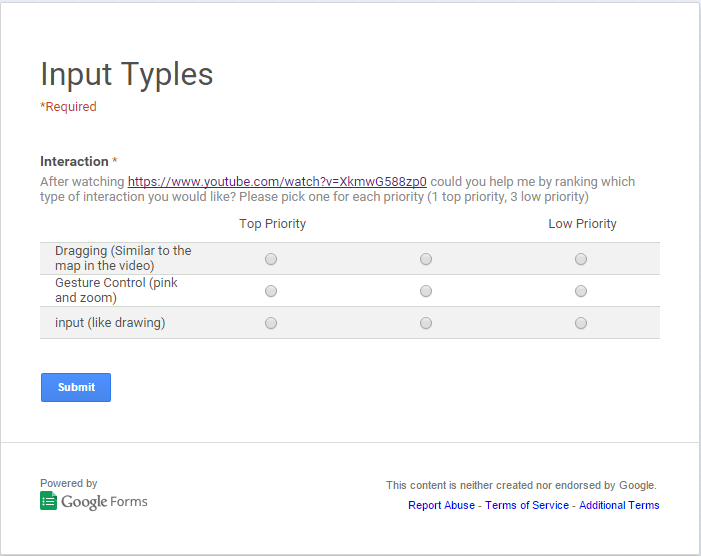
\includegraphics[scale=0.7]{images/googleform}
  \protect\caption{Form to find out preferred interactions} 
  \label{googleform}
\end{figure}


\subsection{Architecture} \label{nocamer_architecture}
\todo[inline]{Implementation.tex: create architecture figure}
 \begin{enumerate}
 \item physical diagram of the table with beacons
 \item software diagram of main activity \-\->library \-\-> kalman filter \-\-> activity
 \end{enumerate}
 I plan to have an arrangement where there is at least are Bluetooth Beacons around the table like show in Figure \_. Using those Beacons as reference nodes I am hoping to calculate the position of a device on the table.

\subsection{Applications}
My research about Bluetooth Low Energy (BLE) technology has shown that there are more than one way to work out the distance between the device emitting the BLE signal and the receiver. 
\begin{enumerate}
\item Accuracy
\item RSSI signal
\end{enumerate}
Most BLE libraries has a method which gives the distance from the beacon to device called Accuracy. Accuracy is a term coined by Apple for their CoreLocation framework to define the distance in meters from the beacon. For Estimote beacons the method is called  \lstinline|computeAccuracy()|. Similar to the Apple function, the calculation done to get this result is hidden by Estimote in their library. However doing more research into some open source libraries \cite{radius-ranging, android_ibeacon_alt} we can make an educated guess that the distance was calculated by observing RSSI and TxPower values at certain distance intervals and making a line of best fit.
The second option is for me to redo the observation to get the resulting RSSI signal and TxPower for each distances and get a line of best fit to work out the distance. However this would mean that my library would be tailored to the set of beacons I have, instead of being a general library. This would be defeating the point of this project. However in section \textbf{do thhis evaluation} we will see how I had to do both type of distancing.

\subsubsection{Distance App} \label{nocamera_distanceapp}
Originally I created an Application which showed the distance from the beacon using \lstinline|computeAccuracy()| method. Figure \ref{distance_app_image} shows the UI for the application. It shows the list, ordered by the distance, of nearby beacons. It also shows other information such as the RSSI value, Transmission Power \ldots
It is a list that keeps updating as new BLE readings come in and and update the RSSI and Transmission power.

\begin{figure}[h]
  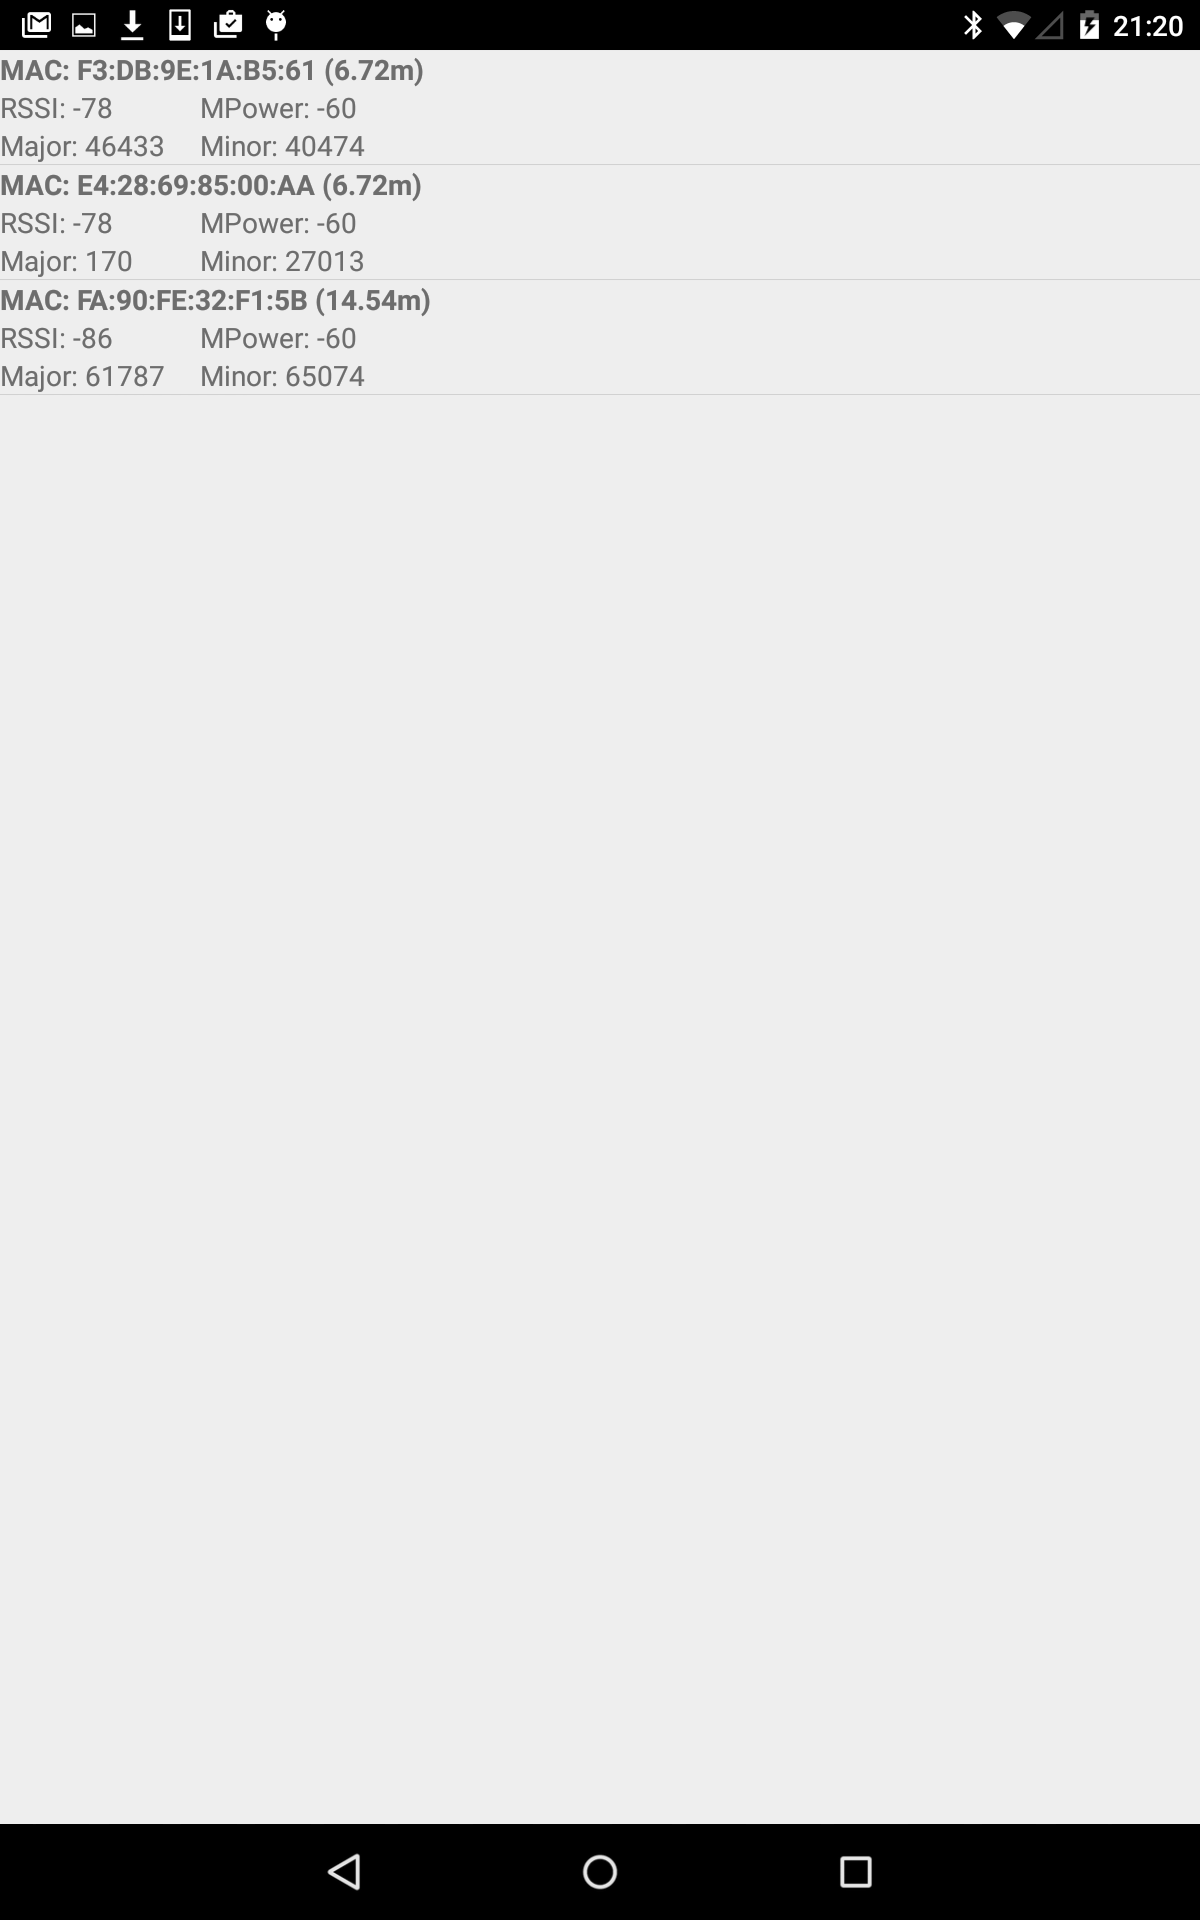
\includegraphics[scale=0.2]{images/distance}
  \protect\caption{Distance App} 
  \label{distance_app_image}
\end{figure}

\subsection{Trilateration} \label{nocamera_trilateration}

By creating the Distance app, I was able to familiarise myself with the Estimote library. This aided me in creating the trilateration part of the library. I decided to stick to a Cartesian coordinate system for my design and created a \lstinline|Position| class which kept track of the x and y position of the devices. I also created a \lstinline|FixedBeacon| class which stored the reference beacon and its location.

Using these new additions I was able to create a method that calculated the position of the receiver on the table. \lstinline|Position calculatePosition(List<FixedBeacon> beaconList)| It requires a list of reference beacons and calculate the distance from those reference beacons. It uses the calculation shown in section \_ to determine the position of the receiver. 
\todo[inline]{evaluate by coordinate system grid!}
Figure \_ shows the output of the calculation which I used for my evaluation in section \_
\begin{figure}[h]
  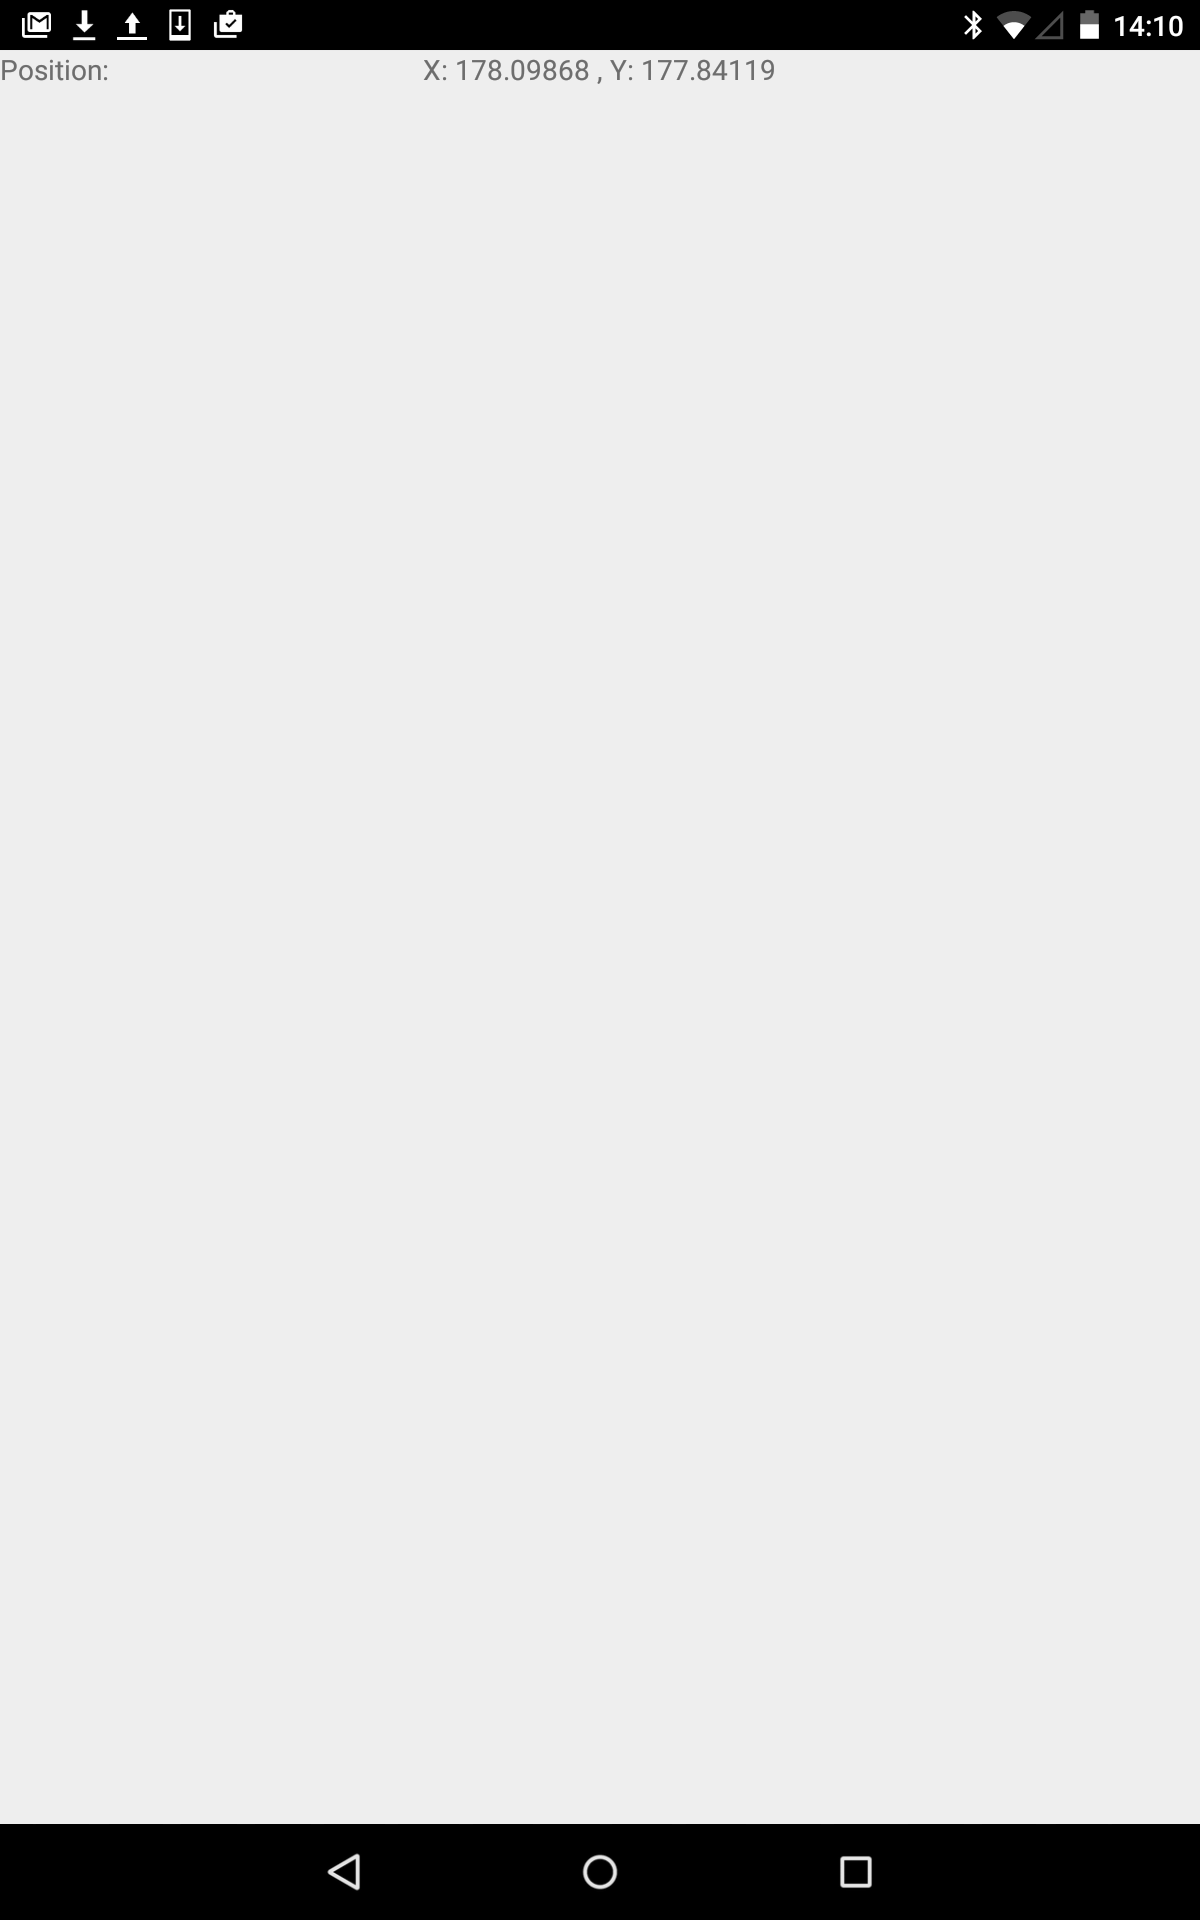
\includegraphics[scale=0.2]{images/trilateration}
  \protect\caption{Trilateration}
  \label{trilateration}
\end{figure}

\subsection{Sensors} \label{nocamera_sensors}
During the implementation and evaluation of the Distance app and Trilateration app, it was clear that something else needs to be combined with BLE for the location system to have chance of being successful. Therefore inspired by the Hybrid sensing method used by HuddleLamp, I decided to add sensor fusion to the positioning algorithm. Having accelerometer to calculate the movement, plus BLE trilateration result together should cancel out some errors given by each other, creating a more accurate positioning system.

After conducting some research into available sensors, the most useful sensor available was the accelerometer. Even though most devices have a gyroscope, the use cases of my library did not require the device to be tilted in any way hence gyroscope was not necessary. 

On a stationary device there is always an acceleration of 1g (9.81 m/s \textsuperscript{2} )
in the z axis due to the effect of gravity on the device. Therefore I needed a calibration step for my sensor where the device polls the sensor for 1 second and use the average values, in all 3 axis, as the zero error. This value will be taken away from any values given by the accelerometer.

As you can see from my research into sensors, in section \nameref{accelerometer}, the process of calculating displacement from accelerometer values is by integrating the values twice. After doing some research into numerical integration methods, the most simple method was the ideal one to use as a proof of concept. I used a simple trapezium rule where I averaged the acceleration value for each second and then integrated it twice by getting the area under the curve for that second twice. by using fixed variables it was possible to change the chunk sizes from 1 second to something smaller if more finer results were required.
Figure \ref{sensor_app_image shows} the UI of the application that showed the accelerometer values in x, y and z axis and also the displacement in the x and y axis.

\begin{figure}[h]
    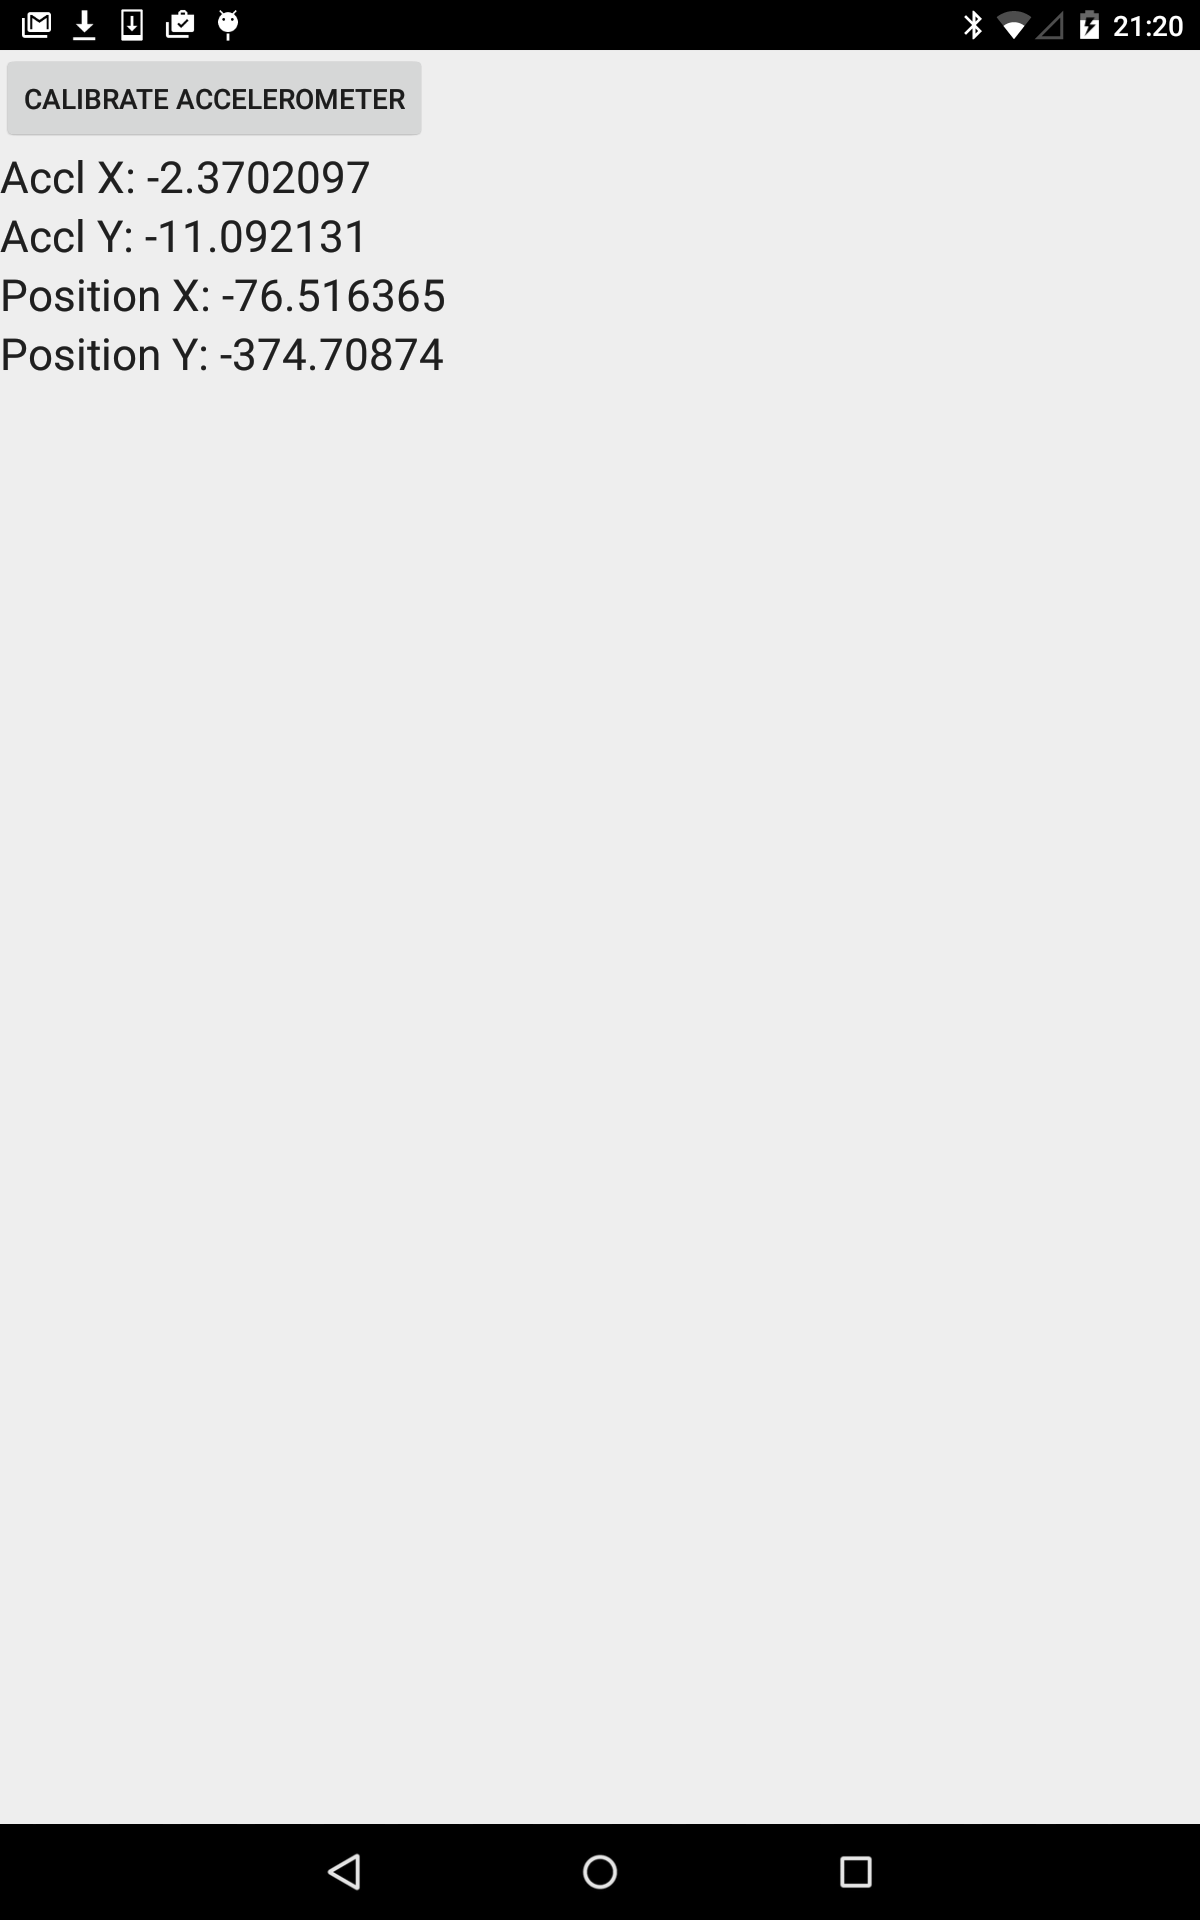
\includegraphics[scale=0.2]{images/sensor}
    \protect\caption{Sensor App} 
    \label{sensor_app_image}
\end{figure}


\subsection{Where is Wally}
One of the main features promoted by the HuddleLamp project was the following the map and where is wally game application that they have created. An application that shows all the advantages of the HuddleLamp project and also an impressive demonstration of the power of the project, I decided to recreate it using my new positioning system. 

During the first iteration of creating my Where is Wally application, I noticed some clear jolting in the images. After careful investigation into the system, there were noticeable noise data that affected the positioning system. This led my investigation into possible noise filtering methods mentioned in \nameref{filter_methods}.

I implemented a Kalman Filter module to my system to reduce the noise in the system. It had a moderate success however in the following evaluation section \_ \_ I would go into detail why this attempt for positioning is not a viable choice for HuddleTable.

\begin{figure}[h]
  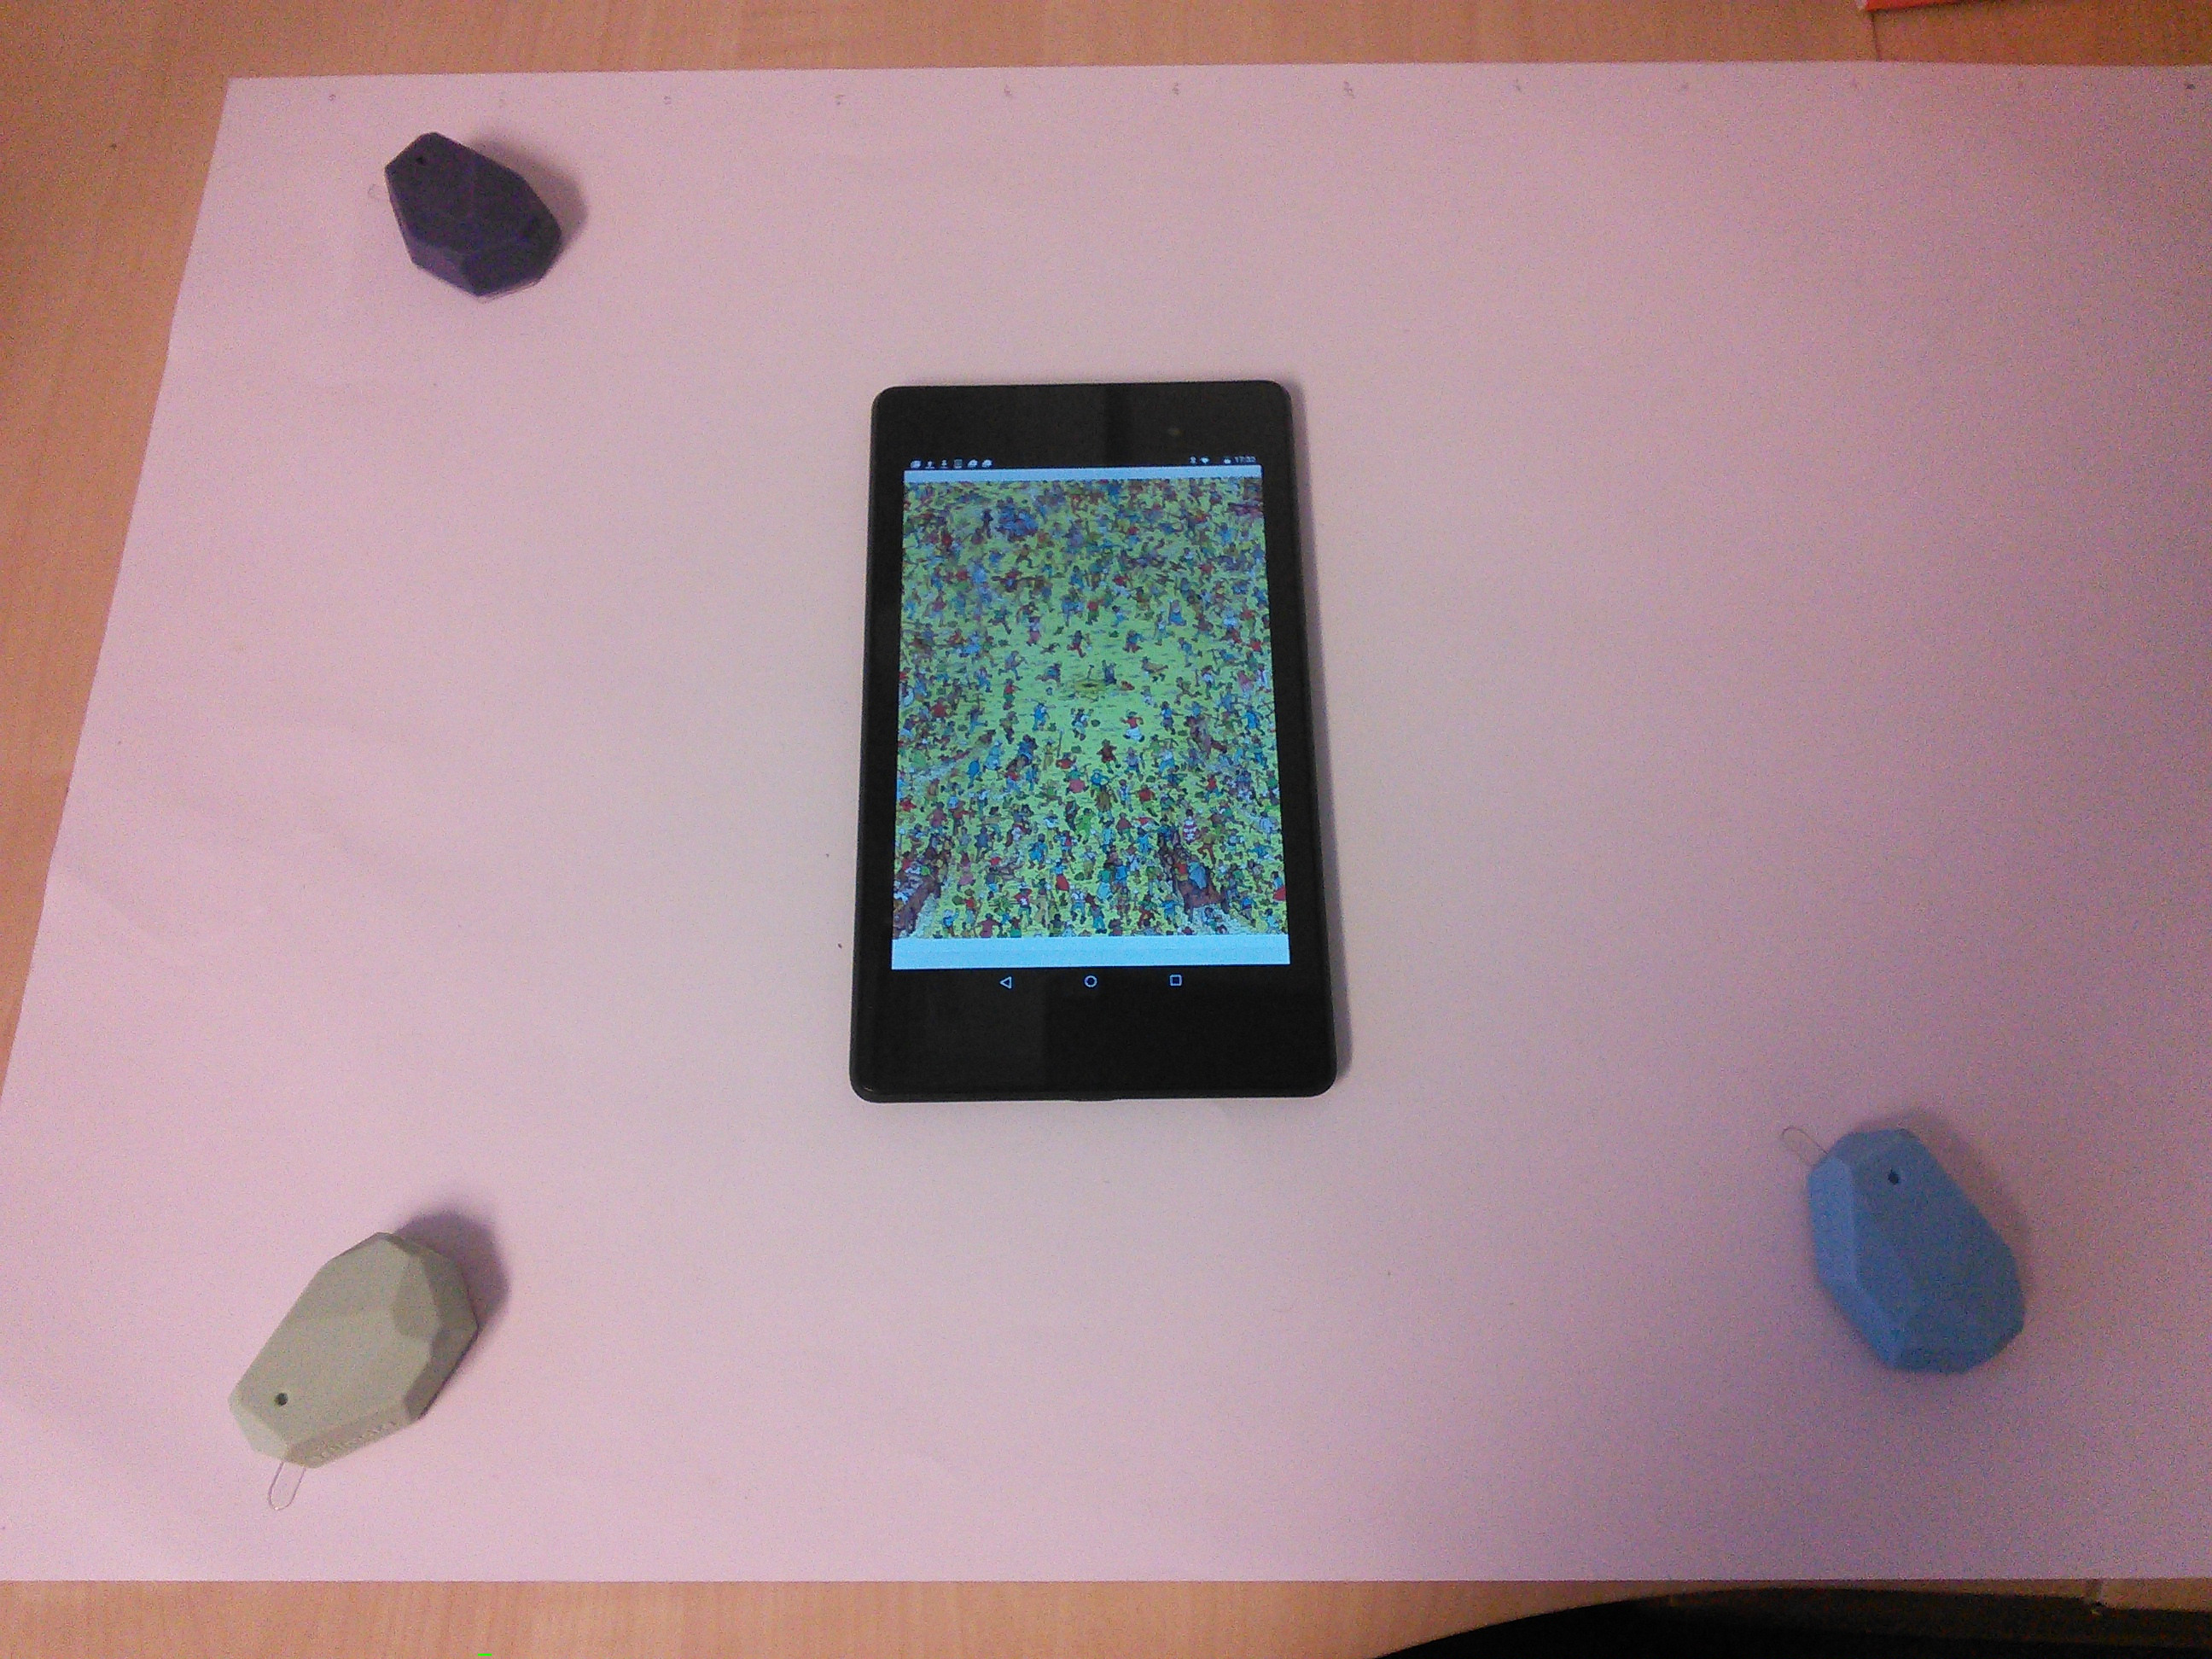
\includegraphics[scale=0.2]{images/setup}
  \protect\caption{Where is Wally App} 
  \label{where_is_wally_setup}
\end{figure}

\subsection{Canvas}
I also created a canvas app which harnessed the full potential of Firebase for this project. This application is similar to a paint application that a user might have. It is aimed at designers wanting to work at particular part of large canvas enabling collaboration with different people to work on the same canvas. Multiple people collaborating on the same document at the same time is one of the problems I wanted to tackle with this project. It was an aspect that was not advertised too much with HuddleLamp and has a potential to be a useful product. 
By utilising the facilities of Firebase and building on their sample project[link to sample project], I was able to create the Canvas Application.


